\documentclass[a4paper,oneside,11pt]{article}
\usepackage{cprform_lett}
\usepackage{amsmath,amstext,amsfonts,amsbsy,amssymb,amscd,bbm,epsfig}
\usepackage{lscape,color,multirow,hyperref, url}
\begin{document}


%%%%%%%%%%%%%%%%%%%%%%%%%%%%%%%%%%%%%%%%%%%%%%%%
% TITLE

\noindent\textsf{\Large A unitary SEIR model}
\vskip 2truemm
\thicktablerule
\vskip 2truemm
\noindent{\large P. Hern\'andez, C. Pena, A. Ramos, J.J. G\'omez-Cadenas\hfill May 2020}
\vskip 10truemm

\section{Introduction}

A burgeoning number of papers attempting to model the dynamics of the COVID-19 pandemic have been published over the last few months \footnote{See for example, the CMMID repository, \url{https://cmmid.github.io/topics/covid19/}}. Among these, a large fraction (\cite{Tang2020, Lin2020, Lopez2020} are just a few examples) are based in more or less complex variants of the classical SEIR (susceptible - infected - recovered) model \cite{Hethcote2000}. 

%A burgeoning number of papers have been published over the last few months in the context of the huge scientific effort to understand the current COVID-19 pandemics \footnote{See for example, the CMMID repository, \url{https://cmmid.github.io/topics/covid19/}}. Among these, a large fraction corresponds to papers attempting to model the dynamics of the epidemics. Two main approaches are used in such modelling efforts. One of them, called ABM (agent based models) is based in a microscopic approach in which individual ``agents'' are allowed to interact under some circumstances ---often described by a spatial grid, a connection network or both--- and the parameters of the infection are obtained as ``macroscopic measurements'' of such interactions (much in the same way that pressure and temperature characterise the interaction of molecules in a gas) \cite{Hunter2017}.  A second approach is based in a set of differential equations (DEM or differential equation models) which purportedly capture the dynamics of the disease\cite{Hethcote2000}. While ABMs are a relatively new approach, DEMs have been used for almost 100 years, since the original formulation of the SIR (susceptible - infected - recovered) model by Kermack and McKendrick \cite{Kermack1927}. In particular, the so called SEIR (susceptible - exposed - infected - recovered) models have been extensively used in epidemiology \cite{Hethcote2000}, both in the past and in the context of the current crisis \cite{Tang2020}.

It has been recently pointed out that such models fail to describe the dynamics of the epidemics, given their inability to properly describe the delay introduced by the incubation time of the disease \cite{fodor2020integral}. As an alternative to SEIR the authors of \cite{fodor2020integral} propose integral equation models. Such models have been considered before (see for example refs.\cite{}).

Prompted by these observations as well as by the imperious need to better understand the tools used for modelling and forecasting, in this paper we study a basic formulation of the SEIR problem, which properly accounts for SEIR delays that we call uSEIR (where the u stands for Unitary) in which a new set of differential equations is deduced which should represent correctly the evolution of an epidemic in the assumption of homogeneity and uniformity of the microscopic parameter, namely: i) number of contacts per unit time, ii) the probability of infection per contact, iii) the incubation time and iv) the recovery time. We demonstrate that the results of uSEIR are reproduced by a microscopic Agent Based Model (ABM) simulation of a fully homogeneous, fully susceptible population in the deterministic limit, e.g, with no stochasticity in the model parameters. 

We also show that stochastic parameters can be incorporated into our equations, and recover the classical SEIR equations in the particular case of exponentially distributed incubation and recovery times. Notice however, that the available data does not support an exponential distribution for these parameters which are usually described by gamma, lognormal or Weibull distributions [REF], none of which are correctly reproduced by classical SEIR. 

The non-uniformity in the infection rate per unit time is more subtle. While the uSEIR equations indicate that the solution should correspond to that in which the infection rate per unit time is the average one, ABM simulations show a large variability and an average that is not well described by any 
SEIR solution. We show that the main effect of this variability is a simple time translation. When the different simulations are shifted to tune their maximums of infected individuals, all the curves fall on a universal curve which is well described by the uSEIR solution. We analyse the origin of this universality, i.e. independence on initial conditions, which derives from an asymptotic solution of the uSEIR equations, which is found to be a logistic curve that depends on the average infection rate. 

The structure of the paper is as follows. In section~\ref{sec:ABM} we briefly describe the agent based simulations that we will use a benchmark.
In sec.~\ref{sec:useir} we present the uSEIR and study the solutions for uniform microscopic parameters. In sec.~\ref{sec:titr} we consider the
non-uniformity in the incubation and recovery times and in sec.~\ref{sec:r} we discuss the non-uniformity in the infection rate per unit time and discuss the universality principle. 

\section{Agent Based Simulations}
\label{sec:ABM}

Agent-based models (ABMs) are microscopic computer simulation based on ``agents'' that can interact with each other, as well as with a computer-defined environment \cite{Hunter2017}. Because agents can make their own decisions in the model based on the rules given to them, ABMs can capture unexpected aggregate phenomena that result from combined individual behaviours in a model. In particular ABMs can incorporate easily stochastic parameters as well as an heterogeneous population.

This paper uses the MESA package \footnote{\url{https://github.com/projectmesa/mesa}} to prepare an ABM simulation of the spread of a epidemic in a fully susceptible, fully homogeneous population. The agents in the model are called ''turtles'', following the nomenclature of the NetLogo \footnote{\url{http://ccl.northwestern.edu/netlogo/index.shtml}} software. The turtle inhabit a square grid and follow a clock which ticks linearly. At each clock tick, all the turtles move in the grid. The sequence in which the turtles move is chosen at random in each tick, and the movement itself is a random step between cells. 

To simulate the evolution of an epidemics the Turtle World is inhabited with $n$ turtles, out of which $n_s$ are susceptible and a small (but as we shall see significant) number, $n_i$ are infectious. At each clock tick infectious (I) turtles have a probability of infecting any susceptible (S) turtle they found in their neighbourhood. Two turtles are considered neighbours if they share the same square. Also, for any given turtle, all turtles located in the eight squares that surround its own are considered neighbours. One can visualise the spacial notion assuming that the squares have a width of 1 m, and thus two turtles closer than 2 m are considered to be neighbours.

The probability for an infectious turtle to infect a susceptible neighbour can be computed from the basic reproductive number, $R_0$, defined as the average number of contacts per unit time during the period of infectiousness. Thus:

\begin{equation}
R_0 = c \times p \times t_r
\end{equation}

Where $c$ is the average number of contacts, $p$ the infection probability, and $t_r$ measures the time of infectiousness. Notice that $t_r$ can be read as a ``recovery time" after which the turtle recovers from the infection, or simply (and more realistically) as a ``removal time'', in which the infected turtle is isolated and therefore can no longer infect others. 

The average number of contacts can be always found by running the simulation without infected turtles. In the case of a fully homogeneous (and large) population, c is simply:

\begin{equation}
c = 9 \frac{n}{a},
\end{equation}
%
where $a$ is the area of the grid cells and 9 accounts for the number of cells that describe the neighbourhood. Therefore, the infection probability can be obtained as: 

\begin{equation}
p = \frac{R_0}{c \cdot t_r}.
\end{equation}

At each step a random number is thrown for each susceptible neighbour of an infected turtle. It the random number is smaller than the infection probability, the turtle becomes exposed and the clock time ($t_e$) is recorded. At each tick all the exposed turtles are examined and eventually turned into infectious when 
$t - t_e > t_i$, where $t$ is the time measure by the World's clock and $t_i$ corresponds to the incubation time. Again, the time at which the transition happens is recorded ($t_i$). The turtle remains infectious until $t - t_i > t_r$, in which case becomes recovered (or removed). 
Notice that the simulation allows the use of uniform or stochastic parameters indistinctly. In the stochastic case each turtle stores its own $t_i, t_r$ which are thrown according to a specified distribution (e.g, Exponential, Gamma, Weibull, etc.). To make the infection probability stochastic, $R_0$ is sampled from a suitable distribution (Poisson, Gamma, Negative binomial, etc.). 

The simulation is run for a number of steps which is typically chosen to be large compared with the ``infection time units'', e.g., if the infection time is measured in days each simulation tick may be 1/5 to /10 of a day. At each step the software records the turtles in each category and thus provides (in the limit of small clock ticks) the functions S(t), E(t), I(t) and R(t), which can be directly compared with the predictions of the solutions of the differential equation models.

\section{Unitary SEIR model}
\label{sec:useir}
We start by considering a model with compartments for susceptible, exposed, infected and recovered individuals at any given time $t$ \cite{}. To be precise we define these categories
as:
\begin{itemize}
\item $S(t)$: number of susceptible individuals at time $t$.
%that is those that can be infected if in contact with an infected 
\item $E(t)$: number of exposed individuals at time $t$, that is those that will become infected after an incubation time,$t_i$. 
%Note that the exposed individuals that will never become infected are part either of susceptible\footnote{Of course there could be individuals that are immunized, but those are out of the count, there are not part of any category that matters here. }
\item $I(t)$: number of individuals at time $t$ that can infect other people. They remain in this category for time $t_r$. This time might be the natural time of recovery or the time it takes to isolate the individual (thus this category is sometimes also dubbed ``removed'' in addition of the more usual ``recovered''). 
% it is in any case the time that it takes for an infected individual to stop infecting, at that moment the individual is declared recovered.
\item $R(t)$: number of recovered (or removed) individuals.
% that contain any individual that was infected in the past and is no longer infectious either because it died, fully recovered or fully isolated so that its probabilty to infect is zero.
\end{itemize}
There is a unitarity condition in this model.  Each individual must be in one of the S,E,I or R categories. Therefore the number of (non-immunised) individuals in the population, $N$, is a constant:
\begin{eqnarray}
S(t)+ E(t)+I(t)+R(t) = N.
\end{eqnarray}
But there must also be a relation between the rates at which these different individuals move from one category to the next. An infection process is that in which an infected individual gets in contact with a susceptible one. Let us call $r_{S\rightarrow E}$ the rate of infection per unit time
per infected individual and per susceptible individual. The number of susceptible individuals gets reduced by those that become exposed between $[t, t+dt]$, that is:
\begin{eqnarray}
d S(t) = - r_{S\rightarrow E} I(t) S(t) dt.
\label{eq:basic}
\end{eqnarray}
In the simplest approximation, if the incubation and recovery time of all individuals have the same values, then we must also have that the individuals that become exposed at time 
$t$ are those that move from category $S\rightarrow E$ at time $t$ minus those that move from $E\rightarrow I$. But the latter must be the ones that entered the exposed category in time $t-t_i$. Therefore we have:
\begin{eqnarray}
d E(t) &=& -d S(t) + d S(t-t_i) \theta(t-t_i) ,\nonumber\\
d I(t) &=& -d S(t-t_i) \theta(t-t_i)+ d S(t-t_i-t_r) \theta(t-t_i-t_r),\nonumber\\
d R(t) &=& - d S(t - t_i - t_r) \theta(t-t_i-t_r).\nonumber
\label{eqs:cor}
\end{eqnarray}

The initial conditions to these equations start with a fixed $N$ and a number of infected individuals at time $t=0$, $I[0]$, so that $S(0) = N-I(0)$, while $E(0)=0$ and $R(0)=0$.  
In the  equations above, the number of initially infected individuals does not recover, but we can easily force this with the substitution in eq.~(\ref{eq:basic}):
\begin{eqnarray}
I(t) \rightarrow \tilde{I}(t) \equiv I(t) - I(0) \theta(t-t_r).
\end{eqnarray}
These equations depend only on three variables, namely $r_{S\rightarrow E}$, $t_i$ and $t_r$, which in principle are the same parameters appearing in the classical SEIR.
The basic reproduction number, $R_0$, defined as the average number of individuals infected by any given infected individual in a fully susceptible population corresponds to the combination:
\begin{eqnarray}
r_{S\rightarrow E} = {R_0\over N t_r}. 
\end{eqnarray}

Since $R_0$ is clearly proportional to $t_r$, it follows that $r_{S\rightarrow E}$ is not. In a microscopic description of the infected process we expect that the rate $r_{S\rightarrow E}$ is basically the product of the number of contacts per unit time and the probability of infection per contact. 

The  formulation of SEIR in the form of eqs.~(\ref{eqs:cor}) we will refer to in the following as uSEIR. Although we are not aware of this precise formulation in the literature, similar ideas of keeping track of delay have been discussed, mostly in the context of SIR in refs. \cite{}.
  
  We can confront both solutions to an agent-based simulations, the details of which are summarized in the Appendix A. 
In Fig.~\ref{fig:fixed} we show the curve for the fraction of infected individuals as a function of time measured from 10 independent simulations in a population of $10^4$ agents with 10 being infected at the initial time, and fixed parameters $t_i$, $t_r$ and $r_{S\rightarrow E}$ for all agents. 
The uSEIR solution agrees very well with the simulations, while the classical SEIR predicts a wider and less pronounced peak. 

\begin{figure}[h!]
  \centering
  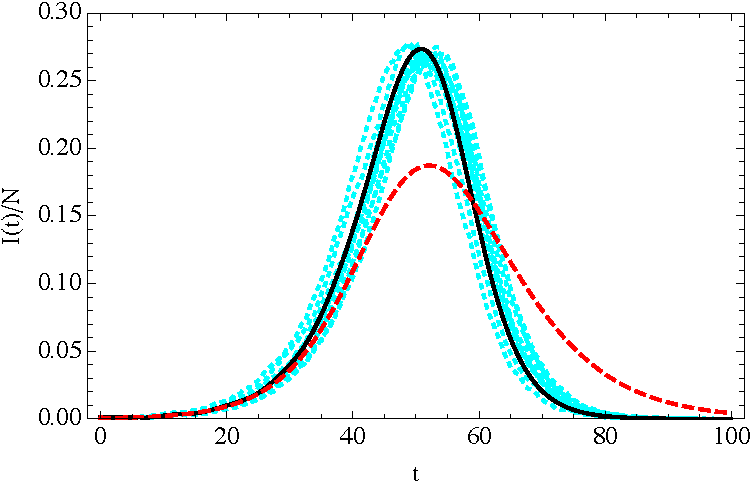
\includegraphics[width=10cm]{fixedraw.pdf}
  \caption{ Curve of the infected individuals as a function of time for the uSEIR (solid-black), classical SEIR (dashed-red) and 10 agent simulations (cyan) in a  population of $N=10^4$ and $I(0)=10$ with $R_0=3.5$, $t_i=5.5$ and $t_r=6.5$.  }
  \label{fig:fixed}
   \end{figure}  
   
  This is maybe not surprising since classical SEIR assumes that the times $t_i$ and $t_e$ are averages, that is they are not uniform in the population. In most realistic cases, not all individuals have the same incubation or recovery period, and certainly not all individuals have the same number of contacts and probability of infection per contact. We consider the effect of these different non-uniformities.
   
\section{Non-uniform $t_i$ and $t_r$ }
\label{sec:titr}

 Non-uniformities can be incorporated in the uSEIR equations by considering different categories of individuals. For example, the population divides   into those with different incubation periods, $t_i^{(i)}$, so we have $S_i(t)$ as the susceptible individuals in the $i$-th category of incubation time. Each category follows its usual progression $S_i\rightarrow E_i \rightarrow I_i \rightarrow R_i$, but the important point to notice is that a given susceptible individual in category $i$ becomes an exposed individual in the same category $i$, but can get infected from any infectious individual in any category, $I_j$. If we assume that the capability to infect per unit time is independent on the category. This means that the number of susceptible individuals in category $i$ change as they become exposed according to:
\begin{eqnarray}
d S_i(t) = - r_{S\rightarrow E} I(t) S_i(t) dt.
\end{eqnarray}
while eqs.~(\ref{eq:cor}) will still be valid for the exposed, infected and recovered in each category $i$, taking the incubation period as that corresponding to this category, $t^{(i)}$. 

Summing over all the categories, the first equation leads to:
\begin{eqnarray}
d S(t) = - r_{S\rightarrow E} \tilde{I}(t) S(t) dt, 
\end{eqnarray}
while in the others we get
\begin{eqnarray}
d E(t) &=& -d S(t) + \sum_i d S(t-t^{(i)}_i) \theta(t-t^{(i)}_i) ,\nonumber\\
d I(t) &=& \sum_i  \left\{-d S(t-t^{(i)}_i) \theta(t-t^{(i)}_i)+ d S(t-t^{(i)}_i-t_r) \theta(t-t^{(i)}_i-t_r)\right\},\nonumber\\
d R(t) &=& \sum_i \left\{- d S(t - t^{(i)}_i - t_r) \theta(t-t^{(i)}_i-t_r)\right\}.\nonumber
\label{eqs:corint}
\end{eqnarray}
Obviously in the limit of $t^{(i)}$ varying continuously the sum becomes an integral
\begin{eqnarray}
\sum_i  (...) \rightarrow \int dt_i P(t_i) (...), \;\;\; \int_0^\infty dt_i P(t_i) = 1.
\end{eqnarray}
We can similarly assume subcategories for varying $t_r$ and the modification would be analogous. 

\subsubsection{Recovering classical SEIR}

The case where the probabilities are exponential, the integro-differential equations can be reduced to regular differential ones, of the classical SEIR type.

 Let's assume 
\begin{eqnarray}
P(t_i) = {1\over \langle t_i\rangle} e^{-t_i/\langle t_i\rangle},
\end{eqnarray}
and define
\begin{eqnarray}
F(t) &\equiv& \int_0^\infty dt_iP(t_i) S'(t-t_i) \theta(t-t_i) = \int_0^t dt_i P(t_i)  S'(t-t_i) \nonumber\\
&=& \int_0^t dz P(t-z) S'(z).
\end{eqnarray}
The derivative of this function is related to that of $E(t)$, using eq.~(\ref{eqs:corint}), 
\begin{eqnarray}
F'(t) = {1\over \langle t_i\rangle} \left({d S\over dt}-F(t)\right) = - {1\over \langle t_i\rangle} {dE\over d t}(t), 
\end{eqnarray}
so up to a constant 
\begin{eqnarray}
F(t) = -{E(t)\over \langle t_i\rangle} +C.
\end{eqnarray}
Since $F(0) = E(0) =0$, the constant must vanish and the equations reduce to:
\begin{eqnarray}
{d S\over dt} &=& - r_{S\rightarrow E} \tilde{I}(t) S(t),\nonumber\\ 
{d E\over dt} &=& -{d S\over d t} - {1 \over \langle t_i\rangle} E(t) ,\nonumber\\
{d I\over dt} &=& {1 \over \langle t_i\rangle} E(t) -{1\over \langle t_i\rangle} E(t-t_r) \theta(t-t_r),\nonumber\\
{d R\over d t} &=&  {1\over  \langle t_i\rangle} E(t-t_r) \theta(t-t_r),\nonumber\\
\end{eqnarray}

If we add also an exponential distribution for the recovery time we need the function
\begin{eqnarray}
G(t) \equiv {1\over \langle t_i\rangle } \int dt_r P(t_r) E(t-t_r) \theta(t-t_r), 
\end{eqnarray}
which for an exponential with average $\langle t_r\rangle$ satisfies
\begin{eqnarray}
G'(t) = {E(t)\over \langle t_r\rangle \langle t_i\rangle} - {G(t)\over  \langle t_r\rangle} = {I'(t)\over \langle t_r \rangle},
\end{eqnarray}
and therefore 
\begin{eqnarray}
G(t) = {I(t)\over \langle t_r \rangle} + C,
\end{eqnarray}
where $C= -I(0)/\langle t_r \rangle$.
Finally we also need to average over $t_r$ in the second term of the function $\tilde{I}$:
\begin{eqnarray}
\int d t_r P(t_r) \tilde{I}(t) = I(t) - I(0) \left(1- e^{-t/\langle t_r\rangle}  \right) \equiv \bar{I}(t)
\end{eqnarray}
 So finally the equations are:
\begin{eqnarray}
{d S\over dt} &=& - r_{S\rightarrow E} \bar{I}(t) S(t),\nonumber\\ 
{d E\over dt} &=& -{d S\over d t} -{1 \over \langle t_i\rangle} E(t) ,\nonumber\\
{d I\over dt} &=& {1 \over \langle t_i\rangle} E(t) - {1\over  \langle t_r \rangle} (I(t) -I(0)),\nonumber\\
{d R\over d t} &=&  {1\over  \langle t_r\rangle} (I(t)-I(0)),\nonumber\\
\label{eqs:seirexp}
\end{eqnarray}
which up to the $I(0)$ are the classical SEIR equations. If $I(0)$ is very small, the extra terms 
 can  be neglected. 

We can easily translate this situation to the agent simulations.  
We start by considering the exponential distributions for $t_i$ and $t_r$, while we maintain the rate of infection constant. The comparison of the SEIR solution of eqs.~(\ref{eqs:seirexp}) and simulations are shown in Fig.~\ref{fig:exp}, where as expected the agreement is good, even if the variance is much larger than in the fixed parameters case.
\begin{figure}[h!]
  \centering
  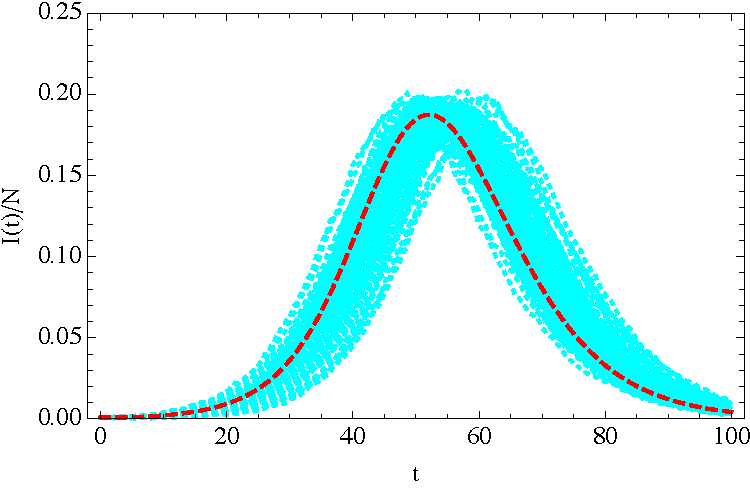
\includegraphics[width=10cm]{expseir.pdf}
  \caption{ Curve of the fraction of infected individuals as a function time of  classical SEIR (dashed-red) of eqs.~(\ref{eqs:seirexp}) and in 100 random agent simulations (cyan) in a  population of $N=10^4$ and $I(0)=10$ with $R_0=3.5$, $\langle t_i\rangle=5.5$ and $\langle t_r\rangle=6.5$.  }
  \label{fig:exp}
   \end{figure}  
   
    Assuming an exponential distribution for the incubation and recovery times are however not realistic. A more realistic distribution seems to be the  gamma distribution, $\Gamma[k,\theta]$ \cite{}. For the Covid19 epidemic the parameters have been estimated to be $(k,\theta) \simeq (5.8, 0.948)$, corresponding to an average $\langle t_i\rangle \simeq 5.5$days. For the recovery time we assume the same distribution with parameters $(6.5,1)$.

We compare the results of the agent simulations with the exponential and gamma distributions in Fig.~\ref{fig:expvsgamma}. We also include the result of solving discretely the eqs.~(\ref{eq:corint}). Classical SEIR does not give a good description of the simulations in this case. 
\begin{figure}[h!]
  \centering
  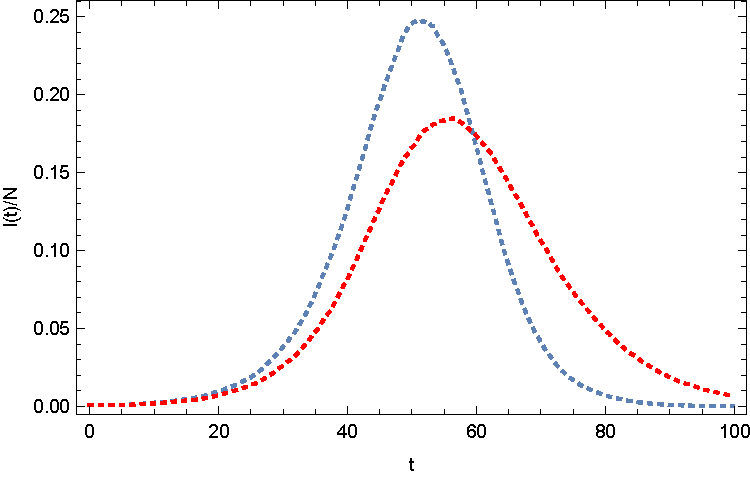
\includegraphics[width=10cm]{expvsgamma.pdf}
  \caption{ Curve of the fraction of infected individuals as a function time from the average of 10 agent simulations with $t_i$ and $t_r$ distributed in the population according to the gamma distributions (blue) and exponentials (red). The simulation has parameters in both cases $N=10^4$ and $I(0)=10$ with $R_0=3.5$, $\langle t_i\rangle=5.5$ and $\langle t_r\rangle=6.5$.  }
  \label{fig:exp}
   \end{figure}  
   
\section{Non-uniform rate and universality }
\label{sec:r}
A different situation is when the rate of infection is non-uniform across the population. It is important to stress that the rate depends on two independent parameters: the number of contacts per infected individual, which critically depends on the clustering properties of the social network,  and the probability of infection per contact. Non-uniformity can originate in either of the two elements, but the implications as we will see are quite different. In this section we will consider the simplest case of a uniform number of contacts, but a non-uniform infecting probability per contact. 

\subsection{Non-uniformity in the probability of infection}
\label{sec:prob}

We could separate the population in individuals that infect others with different rates. The rate might depend on the type of infectious individual and the type of susceptible individual. Defining $r^{j}_{i}$ to be the rate at which an infected individual of type $j$ infects a susceptible individual of type $i$. The equations in this case are:
\begin{eqnarray}
d S_i(t) &=& - \sum_j r^j_{i}  I_j(t) S_i(t) dt, \nonumber\\
d E_i(t) &=& -d S_i(t) + d S_i(t-t_i) \theta(t-t_i) ,\nonumber\\
d I_i(t) &=& -d S_i(t-t_i) \theta(t-t_i)+ d S_i(t-t_i-t_r) \theta(t-t_i-t_r),\nonumber\\
d R_i(t) &=& - d S_i(t - t_i - t_r) \theta(t-t_i-t_r).\nonumber
\end{eqnarray}
where $t_i$ and $t_r$ might also depend on the category.

Assuming that the rates only depend on the type of infecting individual and not on the type of susceptible and, for simplicity $t_i$ and $t_r$ are uniform, only the total number of individuals in each category needs to be evolved. This is the case, because the different categories are in some proportion in the population and we assume the proportion is preserved by
 the initial conditions of the $I_i(0)$ and $S_i(0)$. The equations reduce to the usual ones with a rate that is the weighted average:
 \begin{eqnarray}
 r_{\rm eff} = \sum_i r^i p^i,
 \end{eqnarray}
 where $p^i$ is the proportion of individuals in category $i$.
 
 However, this result seems in conflict with what is found in practice, where the evolution of an epidemic seems very sensitive to the initial conditions, the fraction of immute individuals (herd immunity), the presence of superspreaders, etc. 

Non-uniformity is known to be very important in the evolution of an epidemic. One example is the relevance of the fraction of individuals for which the probability of infecting is zero, which in practice makes them immune. Their presence in a given population implies that the effective number of useful contacts gets reduced. The fraction of the population with zero infecting power is equivalent to the immune fraction. When this fraction is large enough  the epidemic may not start. This is the concept of herd immunity, used to measure the fraction of vaccinated population that can abort an epidemic. A very rough estimate for the fraction of herd immunity, $f_I$, would be
   \begin{eqnarray}
  R_0 (1- f_I)  =1, \;\; f_I= 1-1/R_0. 
   \end{eqnarray} 
   For Covid19, with $R_0 \sim 3$, $f_I \sim 0.7$, that is $70\%$ of the population. One would naively estimate then that in a given epidemic with this herd immunity would result in a 
 fraction of  population that gets infected at some point of 70$\%$, but what we have seen is that the fraction is much larger, both in the SEIR equations as in the simulations. This is because of the time delay in the process, the fraction of recovered individuals grows slowly and is not effective in reducing the growth of the epidemic sufficiently, as if the fraction of immune individuals would be there from the start. 
 
  It has been argued that for Covid19 the distribution of $R_0$ across the population is well described by the negative binomial distribution, $NB[0.16,0.0437]$, which has average 3.5 but a large dispersion. This distribution implies that about $60\%$ of the population would not infect anyone (not far from the naive herd immunity), while there must be few individuals that have a very large rate of infection, the famous superspreaders. 
  
  In Fig.~\ref{fig:turtlesraw} shows the evolution of 100 simulations assuming fixed $t_i$ and $t_r$ while $R_0$ is drawn from a the negative binomial. The average of those histories as well as the result of 
  uSEIR using the average $\langle R_0\rangle$. Clearly the variance if huge, and the average is not a good representation of the individual epidemic histories. The uSEIR curve misses completely the outliers. 
  
 \begin{figure}[h!]
  \centering
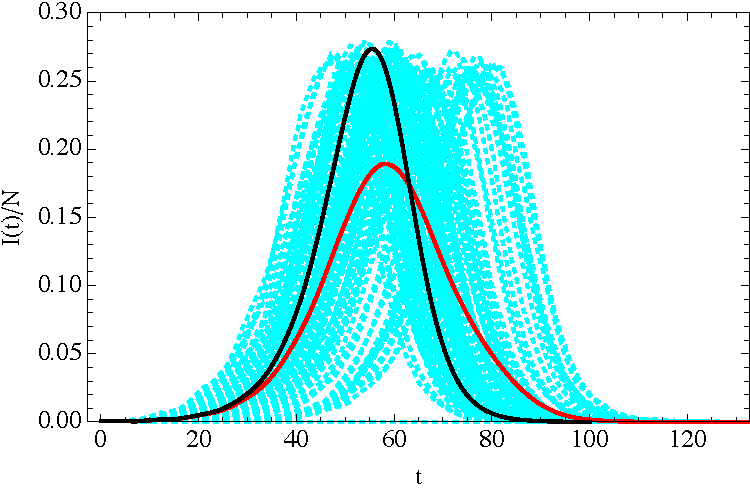
\includegraphics[width=10cm]{turtlesraw.pdf}
  \caption{ Curve of the fraction of infected individuals as a function time from the average of 100 agent simulations with $R_0$ distributed in the population according to negative binomial (cyan) with $t_i$ and $t_r$ are fixed. The average of those histories is the red curve. The simulation has parameters in both cases $N= 2 10^4$ and $I(0)=10$ with $\langle R_0\rangle=3.5$, $t_i=5.5$ and $t_r=6.5$. This is compared to uSEIR (black).}
  \label{fig:turtlesraw}
   \end{figure}
   
   
  There is an interesting observation however. If all the curves are time-translated  to make their maxima coincide, they fall in the uSEIR curve, as shown on the right Fig.~\ref{fig:turtlesshift}.
  \begin{figure}[h!]
  \centering
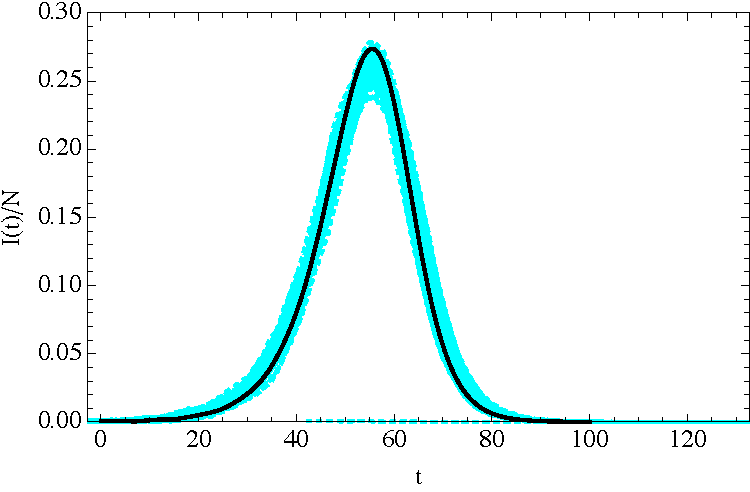
\includegraphics[width=10cm]{turtlesshift.pdf}
  \caption{ The same as in Fig.~{fig:turtles} with the individual ABM simulations time-shifted to keep their maxima invariant and coinciding with maximum of the uSEIR curve.}
  \label{fig:turtlesshift}
   \end{figure}
   
  This fact can be interpreted as follows. The position of the peak is non universal, because it depends very sensitively on the initial conditions, ie. what is the infectious potential of the first infectious agents. Since all epidemic starts with a small number of individuals, we cannot invoke the central limit theorem for the initial stages of an outbreak. These stages have a large variability, however as the exponential growth ensures that the averaging effect of the population starts to be effective. The curve around the maximum is in fact universal in the sense that it depends on the average of the basic parameters and not on the initial conditions, as we now show from the uSEIR equations.
  
  \subsection{Universality and the logistic curve}
  
   We have observed however, that the main effect of the different initial conditions is a temporal shift of the maximum but the shape or the height of the infection curve does not change significantly. This strongly suggest that the equations have a universal solution. We have indeed found it. Let's assume we consider the differential equations eqs.~\ref{} near the maximum of the infection curve $t_{\rm max}$, which will remain as a free parameter. Let's also assume that $t_{\rm max} \gg t_i, t_r$ and let's define the function
 \begin{eqnarray}
 F(t) \equiv S(t) I(t).
 \end{eqnarray} 
 The differential equations for the uSEIR with fixed $t_i$ and $t_r$ and for $t\gg t_i, t_r$:
 \begin{eqnarray}
 {d S \over dt}+{d R\over dt} &=& r F(t-t_i - t_r) - r F(t) \simeq -r (t_i+t_r) \left(F'(t)-{t_i+t_r\over 2} F''(t)\right), \nonumber\\
  {d E \over dt} &=& r (F(t) - F(t-t_i))  \simeq r t_i \left(F'(t)-{t_i\over 2} F''(t)\right) , \nonumber\\
   {d I \over dt} &=& r (F(t-t_i) - F(t-t_i-t_r))  \simeq r t_r \left(F'(t) - \left(t_i+{t_r\over 2}\right) F''(t)\right).
 \end{eqnarray}
 which implies
 \begin{eqnarray}
 S(t)+R(t) &=& C - r (t_i + t_r) \left(F(t)-{t_i+t_r\over 2} F'(t)\right), \nonumber\\
   E(t) &=& C' +r t_i \left( F(t)-{t_i\over 2} F'(t)\right), \nonumber\\
   I(t) &=& C'' +r t_r \left(F(t)-\left(t_i+{t_r\over 2}\right) F'(t)\right). \;\;
 \end{eqnarray}
 Since $I(t) \rightarrow 0, E(t)\rightarrow 0, F(t) = S(t) I(t) \rightarrow 0$ as $t\rightarrow \infty$, it follows that $C'=0, C''=0$ and $C= N$.
 Using the previous equations, it is easy to derive a differential equation for $F(t)$, expanding at linear order in $t_i$ and $t_r$:
  \begin{eqnarray}
 F''(t) - {F'(t)^2\over F(t)} + r^2 {t_r\over t_i+{t_r\over 2}} F(t)^2 = 0. 
 \end{eqnarray}
 We are interested in the solution near the maximum, so we use the initial conditions:
 \begin{eqnarray}
 F'(t_{\rm max}) = 0, \;\;\; F(t_{\rm max}) = F_0.
 \end{eqnarray}
 This non-linear equation has a solution which is given by:
\begin{eqnarray}
F(t) = F_0 \large(1 - \tanh^2\left[ a (t-t_{\rm max})\right]\large),
\label{eq:tanh}
\end{eqnarray} 
with 
\begin{eqnarray}
a\equiv r \sqrt{{t_r F_0\over 2 t_i+t_r}}.
\end{eqnarray}
This is the universal function that drives the evolution of the infected, exposed and susceptible+recovered individuals near the maximum. The maximum of the infected is at $t_{\rm max}-t_i$ for the infected, while the maximum(minimum) for the exposed(susceptible+recovered) is at $t_{\rm max}$. The integral of this function from $[-\infty, \infty]$ is
\begin{eqnarray}
\int_{-\infty}^{\infty} dt F(t) = {2 F_0 \over a}.
\end{eqnarray}
We can also derive the value of the susceptible at $t_{\rm max}$ since
\begin{eqnarray}
S(t_{\rm max}) = {F(t_{\rm max}) \over I(t_{\rm max})} = {1  \over r t_r},
\end{eqnarray}
and the curve of the susceptible can be easily obtained 
\begin{eqnarray}
S(t) = S(t_{\rm max}) - r \int_{t_{\rm max}}^t F(t).
\end{eqnarray}
The total number of susceptible at the end of the epidemic is therefore:
\begin{eqnarray}
S(\infty) = {1\over r t_r } - r {F_0\over a}.
\end{eqnarray}
With this we conclude that the epidemic curve is universal once the value of the maximum position is determined. The value of $F_0$ should also 
depend on the basic parameters and not the initial conditions although 
the precise value is no easy to get. An estimate can be obtained as follows. Near the maximum, and if the incubation and recovery times are sufficiently small we can approximate that $R(t_{\rm max}) \simeq I(t_{\rm max}) + E(t_{\rm max})$, since the infected and exposed quickly recover, using this and the value of $S(t_{\rm max})$ we can estimate $F_0$ to be 
\begin{eqnarray}
F_0 \sim {N-S(t_{\rm max})\over 2 r (t_r +  t_i)}.
\end{eqnarray}
The only dependence on the initial condition remains in $t_{\rm max}$.
In Fig.~\ref{fig:logistic} we compare the numerical solution to the uSEIR equations to the analytic expression of eq.~(\ref{e:tanh}), fixing the parameters $F_0$ and $t_{\rm max}$  the position and height from the numerical solution. Varying the initial conditions, that is the fraction of the number of infected individuals at $t=0$ shifts $t_{\rm max}$ but leaves the curve otherwise invariant. As can be seen the analytical solution describes very well the uSEIR solution. 
\begin{figure}[h!]
  \centering
  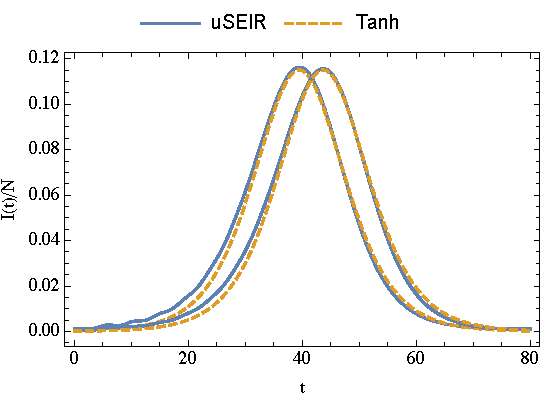
\includegraphics[width=10cm]{logistica.pdf}  
  \caption{Comparison of the results from the uSEIR equations for fixed parameters $R_0=2.1$, $t_i=3$ and $t_r=3$, and the analytical result of  eq.~(\ref{eq:tanh}) with the parameters $F_0$ and $t_{\rm max}$ tuned with the height and position of the peak. The two pairs of solid curves correspond to a fraction of infected individuals of $10^{-3}$ and $5\cdot 10^{-4}$. The two dashed lines are the same function shifted in time.}
  \label{fig:dispersion}
   \end{figure}  
   
   \section{Non-uniform rate: clustering  }
\label{sec:r}

The rate may also be non-uniform because the number of contacts per infecting individual is inhomegeneous in the population. The most efficient way to describe this situation is via the evolution of the epidemic on a network with variable topology \cite{}. 

A network is just a graph \(\{G,E\}\)
consisting on 
nodes \(G=\{n_i\}_{i=1}^N\) and edges linking two nodes, \(E=\{e_{i,j}\}\). We say that
two nodes \(n_a\) and \(n_b\) are connected if \(e_{ab}\in E\). The number
of edges attached to a node \(n_a\) is called its degree and labelled
\(k_a\).

In the context of the spread of an infectious disease, the nodes are
the individuals, and the edges represent the net of individuals 
that have direct contact with him, and are therefore susceptible of being infected by it. The number of edges is therefore the number of contacts. The spread of the disease emerges from the local interaction between nodes via edges. More concretely, in each time step, any infected node $i$ selects randomly one the edges attached to it, for example $e_{i,j}$, and infects the adjacent node, $j$, with a uniform probability $p$. 

 There is empirical experience that realistic networks have some key
properties that might be relevant for the rate of spread of an epidemic. 
They are scale-free, that is the distribution of the degree (i.e. the number of contacts per node) has the form \(P(k)\sim k^{-\gamma}\). In such networks the dispersion of the number of edges is large. Realistic networks have a large clustering coefficient, which measures the probability that two nodes connected to a third, are also connected among themselves. Intuitively, it is clear that the spread of a disease in a network with large clustering is less efficient, because it is difficult for the infectious agent to jump between clusters. 

We will concentrate on a particular
one-parameter family of scale-free networks described by Klemm and Eguiluz (KE) 
\cite{Klemm_2002}, where the average local clustering can be tuned with the free parameter, \(\mu\). In Fig.~\ref{fig:KE} we show the distribution of $k$ on the KE networks varying $\mu$, compared to a random network with no clustering . Even if two networks share the number of nodes, edges and the degree distribution, they can look very different if the average clustering coefficient, $C_i$ is different, with
\begin{eqnarray}
C_i \equiv \frac{2|\{e_{jk}\setminus e_{ji},e_{ki},e_{jk}\in E\}|}{k_i(k_i-1)}\,.
\end{eqnarray}
In Figs.~\ref{fig:networks} two networks with different $C_i$ are shown.

\begin{figure}[htbp]
\centering
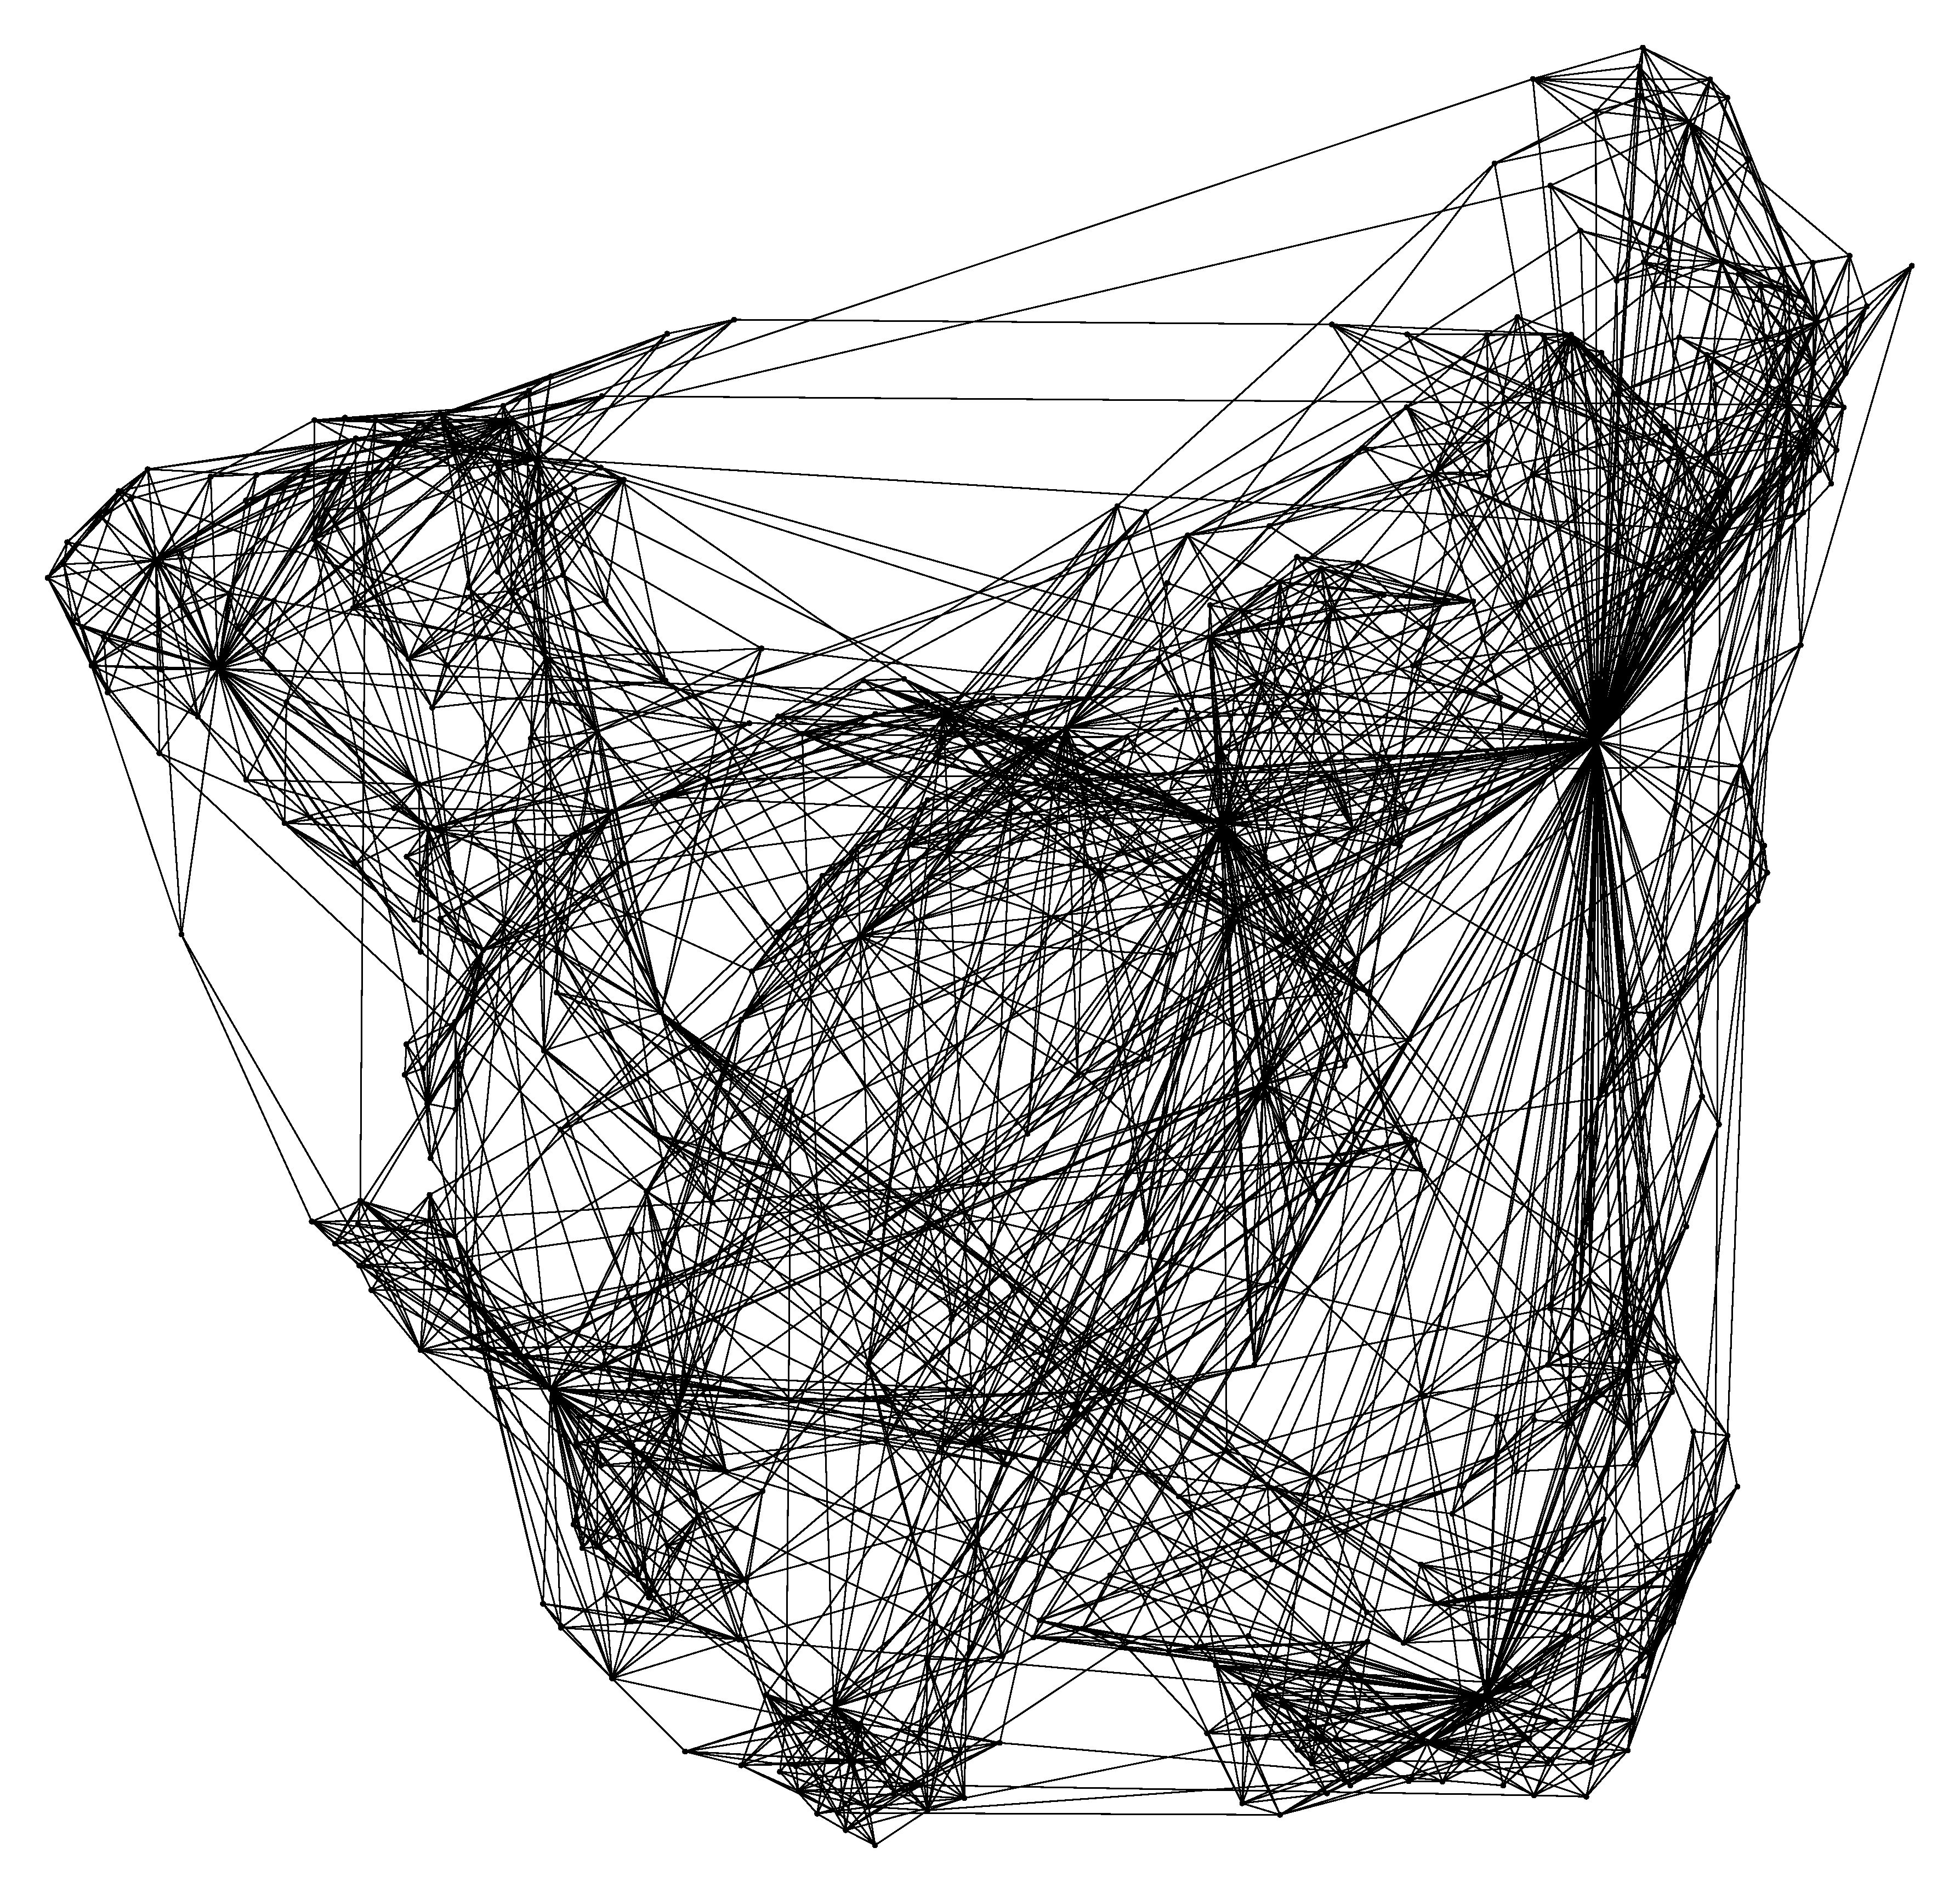
\includegraphics[width=.45\linewidth]{ke_05_09.pdf} 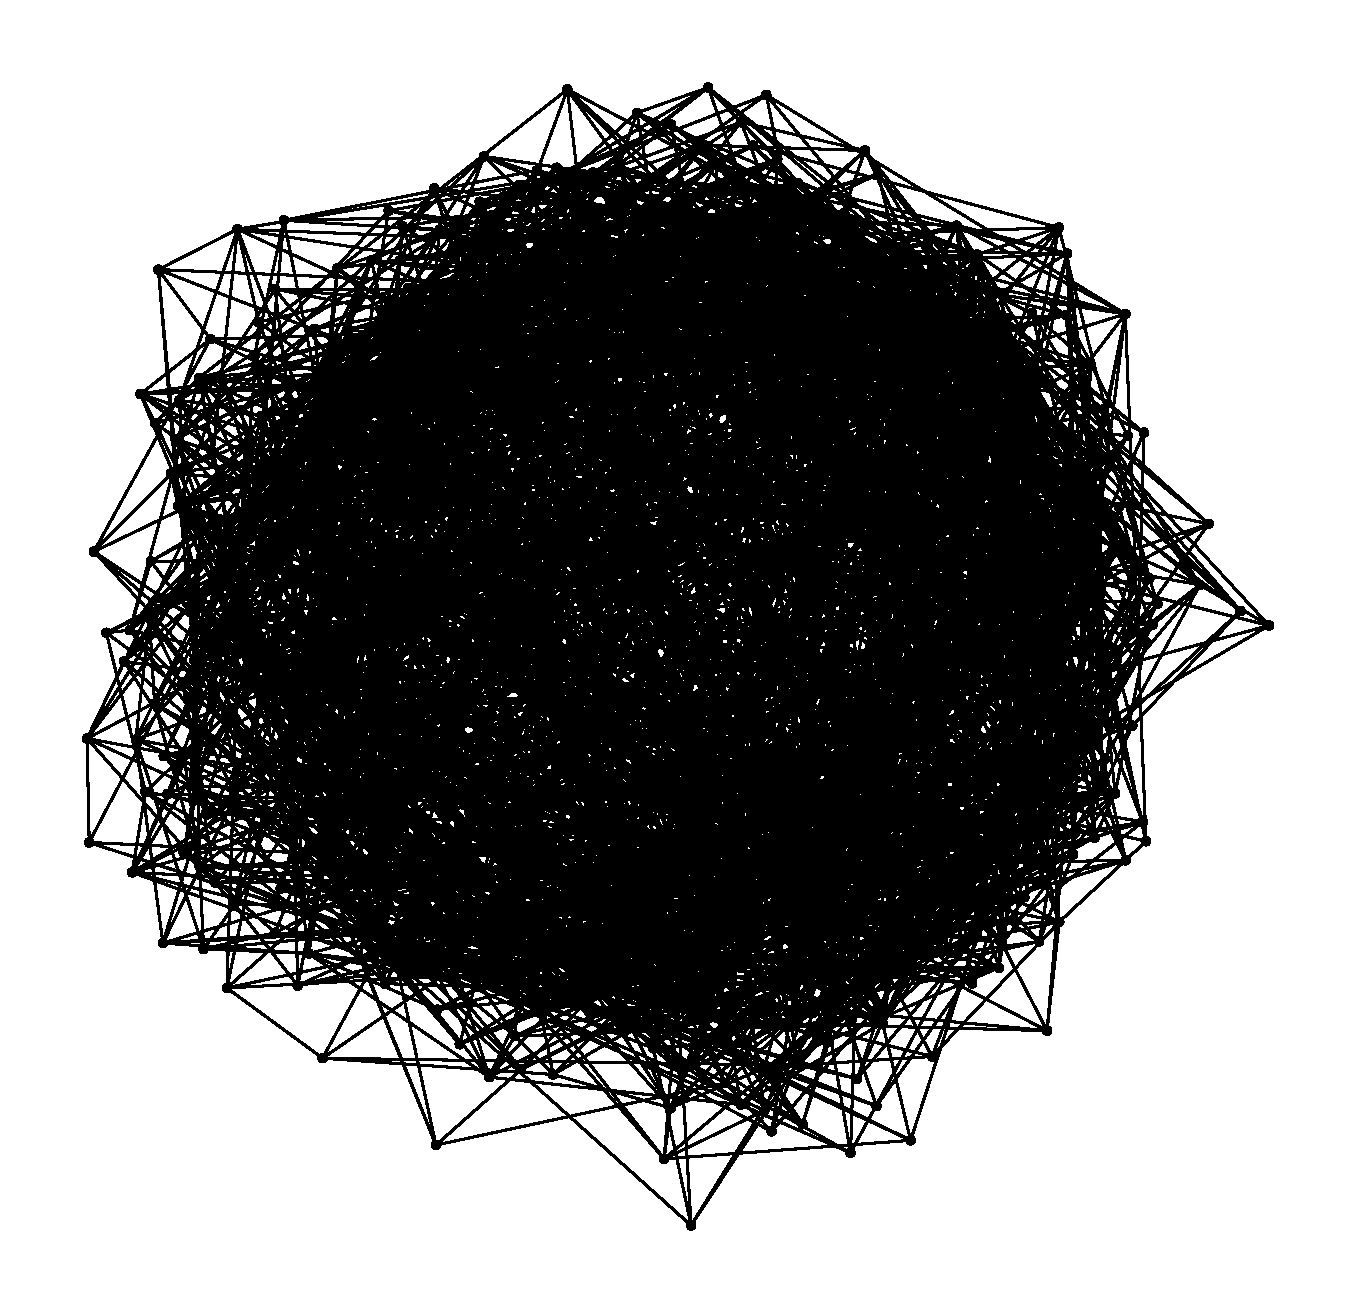
\includegraphics[width=.45\linewidth]{ke_05_01.pdf}
\caption{Two examples of KE network with 500 nodes, mean degree \(\langle k \rangle=9.93\) and different clustering: \(\langle C_i \rangle = 0.5\) (\(\mu=0.9\)) (Left) and \(\langle C_i \rangle = 0.07\) ( \(\mu=0.1\)) (Right)}
\end{figure}

\subsection{Simulating the epidemics evolution on a network}

The evolution of the disease in any of the networks is monitored by the number of nodes in states $S, E, I, R$ at any step. Starting with a fraction of  infected nodes, the infected nodes proceed to infect other susceptible nodes with the rules described above,  changing their state to $E$. The nodes in state $E$ move to state $I$, with a delay given by a fixed incubation time. In state $I$ the start infecting susceptibles connected to them, and remain doing so before a the removal time, $t_r$, elapses at which point they change state to $R$ and remain there. 

If Fig.~\ref{fig:useirvsnet} we show the evolution of infected individuals as a function of time for various networks with different clustering properties. The simulation points correspond to the average of xx simulations after a shift of $t_{\rm max}$ to match the position of the maxima. We find very good agreement with the universal behaviour that derives from uSEIR, eq.~(\ref{eq:tanh}), in all cases. However the fitted value of $a$ changes with the topology of the network. In Fig.~\ref{} we show the dependence of
$a$ on the clustering parameter $\mu$. This is in clear contrast with the situation we observed for the inhomogenities in the probability of infection, where the curves matched the average value of the microscopic parameter $a$. The networks we are considering have all the same average degree and therefore the same average number of contacts. Since the probability of infection is also constant, this means that the average 
microscopic $a$ is the same, but the {\it effective} one varies with the clustering. 
\begin{figure}[htbp]
\centering
 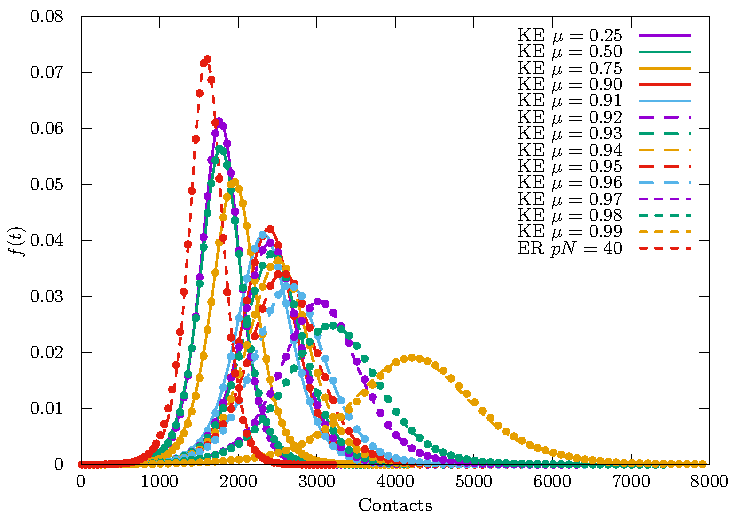
\includegraphics[width=.8\linewidth]{uSEIR.pdf}
\caption{Average fraction of infected nodes with time in networks with equal average degree but different clustering properties. The curves are fits  to eq.~(\ref{eq:tanh}), leaving $a$, $F_0$ and $t_{\rm max}$ as free parameters. }
\end{figure}

The clustering property of the network affects the speed of propagation of the disease in the population, much like the index of refraction, affects the velocity of propagation of a particle in a medium. This was observed before ?? \cite{}. 



\section{Conclusions}

\section*{Appendix A} 

Numerical solution of uSEIR equations.



  
%\begin{figure}[h!]
%  \centering
%  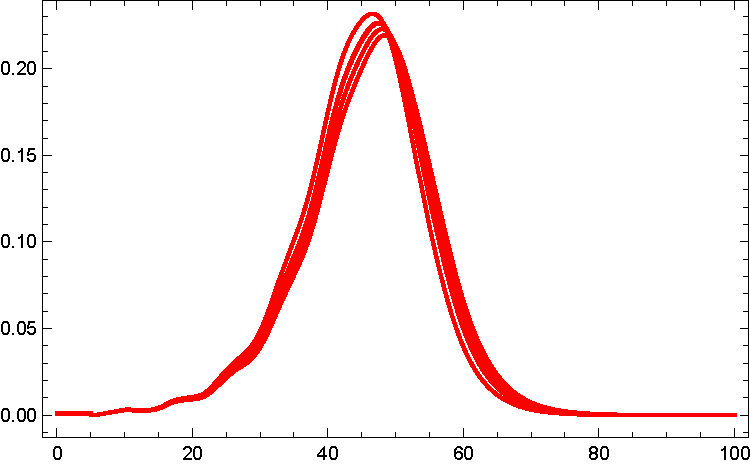
\includegraphics[width=7cm]{NBdisR0.pdf}   %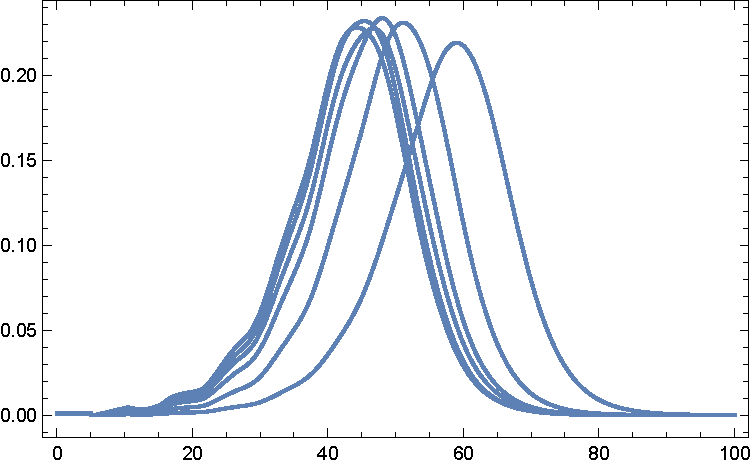
\includegraphics[width=7cm]{NBdisR00.pdf}
%  \caption{ Left: Curve of the fraction of infected individuals as a %function time resulting from the uSEIR equations  for fixed $t_i =5.5$ and $t_r=5$ with $N=10^4$ and $I(0)=10$ and $R_0$ drawn from the average of the $N$ population. Right: the same but assuming that the rate  $R_0$ for $t<t_r$  is the average over the 10 individuals that start the epidemic and for later time the rate turns to the average. }
%  \label{fig:dispersion}
%   \end{figure}  
   
 
 
 
%\subsection{Time-varying Parameters}
\section{Conclusions}

%\end{document}
%
%\title{SEIR de andar por casa}
%
%A ver, he estado intentado entender el asunto del tiempo de incubaci\'on y de recuperaci\'on en el SEIR y he llegado a la conclusi\'on de que 
%no lo entiendo, en particular que el n\'umero de infectados en tiempo $t$ sea proporcional al n\'umero de expuestos en tiempo $t$...
%
%Si hago las siguientes asumptions:
%\begin{itemize}
%\item hay un tiempo de incubaci\'on $t_i$ igual para todos los individuos
%\item hay un tiempo de recuperaci\'on $t_r$ igual para todos los individuos
%\end{itemize}
%las ecuaciones que para mí tendrían sentido, en términos de unitariedad, son las siguientes:
%\begin{eqnarray}
%{d S\over d t} & = & - \alpha I(t) S(t),\\
%{d E\over d t} & = & \alpha I(t) S(t) - \alpha I(t-t_i) S(t-t_i)  \theta(t-t_i),\\
%{d I\over d t} & = & \alpha I(t-t_i) S(t-t_i) \theta(t-t_i) - \alpha I(t-t_i-t_r) S(t-t_i-t_r)  \theta(t-t_i-t_r),\\
%{d R\over d t} & = & \alpha I(t-t_i-t_r) S(t-t_i-t_r)  \theta(t-t_i-t_r),\\
%\end{eqnarray}
%donde
%\begin{eqnarray}
%\alpha= {R_0\over N t_r} 
%\end{eqnarray}
%En esencia, los que pasan a infectados en tiempo $t$ son los que estaban pasando a expuestos a tiempo $t-t_i$, y los que pasan 
%a recuperados a tiempo $t$ los que estaban pasando a expuestos a tiempo $t-t_i-t_r$...
%
%Comparo con la soluci\'on SEIR (dashed) con supuestamente los mismos par\'ametros donde $t_i$ y $t_r$ si entiendo bien aparecen en los
%rates. Asumo $S[0] = 1000, I[0] =1,  t_r=15,  t_i=5 , \alpha=R_0/t_r = 1/5$.
% \begin{figure}[h!]
%  \centering
%  \includegraphics[width=8cm]{sir.pdf}
%   \end{figure}  
%
%Hay que hacer una pequeña modificaci\'on para que los que est\'an infectados al principio $I[0] = I_0$ decaigan tambi\'en (si no se quedan en el limbo):
%\begin{eqnarray}
%{d S\over d t} & = & - \alpha \tilde{I}(t) S(t),\\
%{d E\over d t} & = & \alpha \tilde{I}(t) S(t) - \alpha \tilde{I}(t-t_i) S(t-t_i)  \theta(t-t_i),\\
%{d I\over d t} & = & \alpha \tilde{I}(t-t_i) S(t-t_i) \theta(t-t_i) - \alpha \tilde{I}(t-t_i-t_r) S(t-t_i-t_r)  \theta(t-t_i-t_r),\\
%{d R\over d t} & = & \alpha \tilde{I}(t-t_i-t_r) S(t-t_i-t_r)  \theta(t-t_i-t_r),\\
%\end{eqnarray}
%with
%\begin{eqnarray}
%\tilde{I}(t) \equiv I(t) - I(0) \theta(t-t_r)\
%\end{eqnarray}
%
%Para incluir una estocasticidad en el valor de $t_i$, a\~nadimos una integral en los t\'erminos de la derecha de la forma
%\begin{eqnarray}
%\int dt_i P(t_i) (...),
%\end{eqnarray}
%donde asumimos un distribuci\'on $\gamma$ con $(k,\theta)=(5.8,0.948)$ \cite{}. En la pr\'actica Mathem\'atica no sabe hacer esto, as\'{\i} que 
%divido la distribuci\'on en tres rangos $[0,t_1], [t_1,t_2], [t_2,\infty]$, con probabilidad $\sim 0.3$ cada uno,  donde tomo la media $\langle t_i\rangle_{1-3}$ en el intervalo y hago la integral como suma 
%de tres t\'erminos:
%\begin{eqnarray}
%\int d t_i P(t_i) f(t_i) \simeq \sum_k f(\langle t_i\rangle_k) \int_{t_k^{min}} ^{t_k^{max}}  P(t_i) 
%\end{eqnarray}
%The comparison of the evolution of infected with an average $t_i$ or an integral with three ranges is shown in \ref{fig:comp}
% \begin{figure}[h!]
%  \centering
%  \includegraphics[width=8cm]{deltavs3.pdf}
%  \label{fig:comp}
%  \caption{Unitary SEIR with fixed $t_i=5.5$ (solid) or with three ranges according to the $\gamma$ distribution (dashed).}
%   \end{figure}  
%We can do the same for changing $t_r$ instead, while any possible change to $\alpha$ of this form would not modify the result for fixed $\langle \alpha\rangle$. 
%
%What is clear is that if we start with the measured $R_0$, unless there is a change with time of $\alpha$ there 
%
\bibliographystyle{unsrt}
\bibliography{refs}
\end{document}

